\chapter{Analisi dei costi}
\label{cap:analisi-costi}
\intro{In questo capitolo verrà descritta l'analisi dei costi effettuata sul progetto.}\\

\section{Introduzione}
\label{sec:introduzione}
L'analisi dei costi è un'attività fondamentale per la realizzazione di un progetto, in quanto permette di stimare il costo totale del progetto e di conseguenza il budget necessario per la sua realizzazione e mantenimento.\\
Verranno descritti i principali costi di mantenimento della WebApp, in particolare verranno analizzati i costi di hosting, di distribuzione e caricamento dei video, che essendo basata sull'utilizzo dell'infrastruttura di Azure, sono i costi principali.\\

\subsection{Costi di hosting}
\label{subsec:costi-hosting}
I costi di hosting sono i costi necessari per mantenere la WebApp online, in particolare sono i costi per l'hosting del backend e del frontend. Durante lo sviluppo del PoC, è stato utilizzato un piano di distribuzione gratuito, che permette di distribuire l'applicazione senza costi aggiuntivi con delle limitazioni sulle operazioni che possono essere effettuate. In caso di produzione dell'applicazione, è necessario considerare dei costi per l'hosting, in quanto il piano gratuito non è adatto per l'hosting di un'applicazione in produzione. Azure offre diversi piani di hosting, che differiscono per le risorse disponibili e per il costo. Il piano più adatto per una WebApp di questo tipo in produzione è il piano Premium, che offre un numero illimitato di App, 250GB di spazio di archiviazione, fino a 30 istanze e la possibilità di utilizzare un dominio personalizzato e l'autoscale ad un costo di 0.184€/h, ovvero 4.416€/giorno.\\
\subsection{Costi di codifica}
I costi di codifica sono i costi necessari per effettuare la codifica dei video caricati nei vari formati, sono riportati nella seguente tabella //TODO: link alla tabella.
Per lo sviluppo del PoC è stata utilizzata la codifica in HD, idealmente per l'app in produzione si utilizzerà la codifica in 4K visto l'evoluzione della disponibilità di rete e dell'aumento delle risoluzioni dei dispositivi sempre più accessibili.

\subsection{Costi di trasferimento}
Azure Media Service prevede un costo fisso per ogni GB trasferito tra le stesse zone di distribuzione, ovvero che se il file richiesto si trova in Europa e anche il richiedente avrà un costo di 0.010€/GB mentre se si trovano in zone differenti i costi aumentano come riportato nella seguente tabella //TODO: link alla tabella

\subsection{Costi di distribuzione}
\label{subsec:costi-distribuzione}
I costi di distribuzione sono i costi necessari per la distribuzione in streaming dei contenuti multimediali. Durante lo sviluppo del PoC è stato utilizzato lo Standard Streaming Endpoint, che ha un Bandwidth di 600Mbps a un costo di 1.9088€/giorno, ovvero 59.172€/mese, che è il piano più basso disponibile, permette una distribuzione a circa 171 utenti contemporaneamente con un utilizzo medio di 3.5Mbps per utente. È limitante in quanto, una volta saturato il Bandwidth, non permette la scalabilità automatica, che causerebbe buffering ai client, e bisognerebbe passare ad un piano superiore.\\

\section{Consuntivo preventivato}
In caso di produzione dell'applicazione, è necessario stimare il numero di utenti che utilizzeranno l'applicazione per poter scegliere i piani più adatti e avere una stima dei costi circa accurata.\\
È stato realizzato un modello matematico che stima in base ai dati messi in input come numero di utenti iscritti, percentuale di utenti attivi giornalmente, durata media di visione per utente, orari e ampiezza del picco, qualità video richiesta, il costo medio giornaliero dell'applicazione, che prevede i costi di codifica, trasferimento e distribuzione, vengono riportati tre scenari.
Per congruenza dei dati, ogni scenario prevede gli stessi dati in input tranne che per il numero di iscritti:

\begin{table}[H]
    \label{tab:dati-input}
    \begin{tabularx}{\textwidth}{|c|X|}
        \hline
        \textbf{Oggetto} & \textbf{Valore} \\\hline
        
        \textbf{Percentuale utenti iscritti} & {10\%} \\ 
        \hline
        \textbf{Durata media visualizzazioni in secondi} & {300s} \\ 
        \hline
        \textbf{Percentuale richieste HD} & {50\%}\\
        \hline
        \textbf{Percentuale richieste FHD} & {50\%}\\  
        \hline
        \textbf{Banda media HD} & {4Mbps}\\  
        \hline
        \textbf{Banda media FHD} & {7Mbps}\\  
        \hline
        \textbf{Costo per singolo Premium Unit Streaming} & {0.17€}\\  
        \hline
        \textbf{Costo per GB trasferito} & {0.010€}\\  
        \hline
    \end{tabularx}
    \caption{Tabella di dati in input}

\end{table}

\subsubsection{Caso 10000 utenti iscritti}
Per il primo scenario, si è scelto di considerare 10000 utenti iscritti, che è un numero ragionevole per una WebApp di questo tipo all'inizio della sua vita.\\
\begin{table}[H]
    \label{tab:costi-10000}
    \begin{tabularx}{\textwidth}{|c|X|}
        \hline
        \textbf{Oggetto} & \textbf{Valore} \\\hline
        
        \textbf{Costo App Service Giornaliero} & {4.416€} \\ 
        \hline
        \textbf{GB usati giornalmente} & {201 GB} \\ 
        \hline
        \textbf{Costo di trasferimento} & {2.014€}\\
        \hline
        \textbf{Costo totale di Premium Unit Streaming} & {4.17€}\\  
        \hline
        \textbf{Totale giornaliero} & {10.60€}\\  
        \hline
        \textbf{Totale mensile} & {328.45€}\\  
        \hline
        \textbf{Totale annuale} & {3.867.23€}\\  
        \hline
    \end{tabularx}
    \caption{Tabella costi con 10000 utenti iscritti}
\end{table}
\begin{figure}[H]
    \centering
    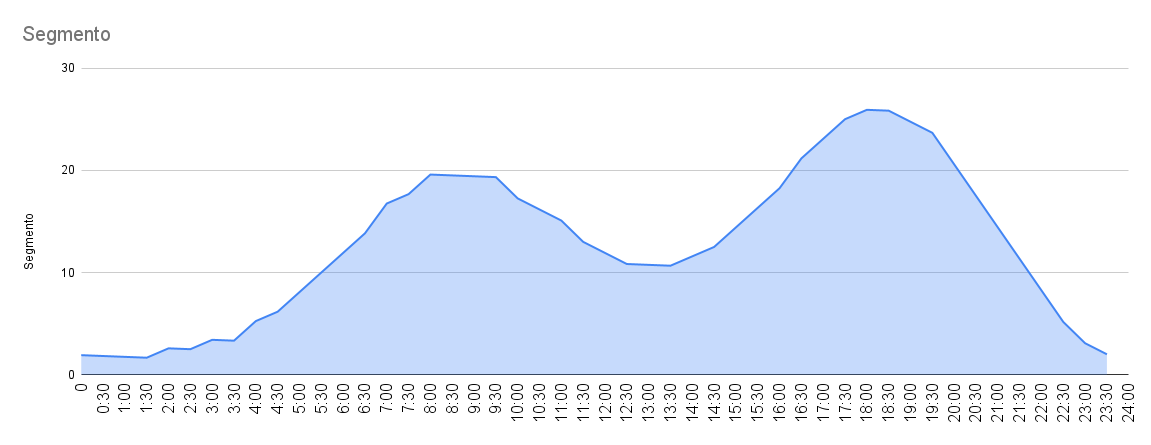
\includegraphics[scale=0.25]{images/costi/10kuser.png}
    \caption{Grafico utenti/orario con 10000 utenti iscritti}
    \label{fig:costi-10000}
\end{figure}
\subsubsection{Caso 100000 utenti iscritti}
Per il secondo scenario, si è scelto di considerare 100000 utenti iscritti, che è un buon numero di utenti per una WebApp di questo tipo in caso iniziasse a crescere.\\
\begin{table}[H]
    \label{tab:costi-100000}
    \begin{tabularx}{\textwidth}{|c|X|}
        \hline
        \textbf{Oggetto} & \textbf{Valore} \\\hline
        
        \textbf{Costo App Service Giornaliero} & {4.416€} \\ 
        \hline
        \textbf{GB usati giornalmente} & {2014 GB} \\ 
        \hline
        \textbf{Costo di trasferimento} & {20.142€}\\
        \hline
        \textbf{Costo totale di Premium Unit Streaming} & {7.02€}\\  
        \hline
        \textbf{Totale giornaliero} & {31.57€}\\  
        \hline
        \textbf{Totale mensile} & {978.80€}\\  
        \hline
        \textbf{Totale annuale} & {11524.64€}\\  
        \hline
    \end{tabularx}
    \caption{Tabella costi con 100000 utenti iscritti}
\end{table}
\begin{figure}[H]
    \centering
    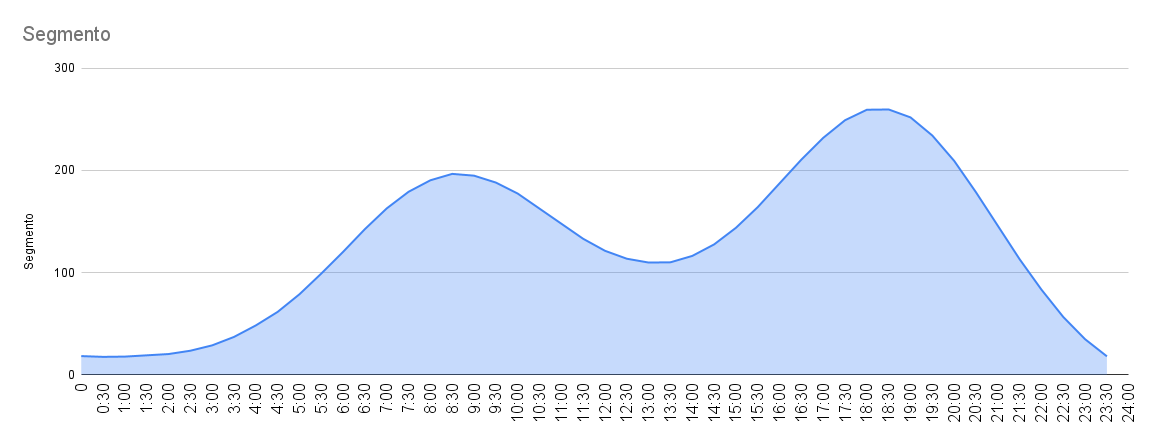
\includegraphics[scale=0.25]{images/costi/100kuser.png}
    \caption{Grafico utenti/orario con 100000 utenti iscritti}
    \label{fig:costi-100000}
\end{figure}

\subsubsection{Caso 1000000 utenti iscritti}
Per il terzo scenario, si è scelto di considerare 1000000 utenti iscritti, che è un numero importante di utenti in caso la WebApp avesse un grande successo.\\
\begin{table}[H]
    \label{tab:costi-1000000}
    \begin{tabularx}{\textwidth}{|c|X|}
        \hline
        \textbf{Oggetto} & \textbf{Valore} \\\hline
        
        \textbf{Costo App Service Giornaliero} & {4.416€} \\ 
        \hline
        \textbf{GB usati giornalmente} & {20142 GB} \\ 
        \hline
        \textbf{Costo di trasferimento} & {201.416€}\\
        \hline
        \textbf{Costo totale di Premium Unit Streaming} & {11.13€}\\  
        \hline
        \textbf{Totale giornaliero} & {216.96€}\\  
        \hline
        \textbf{Totale mensile} & {6725.85€}\\  
        \hline
        \textbf{Totale annuale} & {79191.41€}\\  
        \hline
    \end{tabularx}
    \caption{Tabella costi con 1000000 utenti iscritti}
\end{table}
\begin{figure}[H]
    \centering
    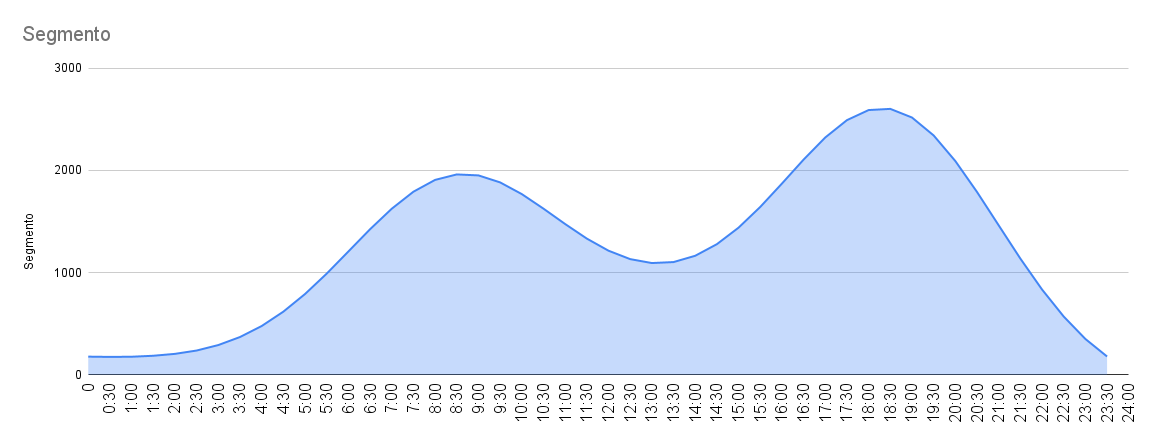
\includegraphics[scale=0.25]{images/costi/1000kuser.png}
    \caption{Grafico utenti/orario con 1000000 utenti iscritti}
    \label{fig:costi-1000000}
\end{figure}